% NIH Grant Proposal for the Specific Aims and Research Plan Sections
%----------------------------------------------------------------------------------------
%	PACKAGES AND OTHER DOCUMENT CONFIGURATIONS
%----------------------------------------------------------------------------------------

\documentclass[11pt,notitlepage]{article}

% A note on fonts: As of 2013, NIH allows Georgia, Arial, Helvetica, and Palatino Linotype. LaTeX doesn't have Georgia or Arial built in; you can try to come up with your own solution if you wish to use those fonts. Here, Palatino & Helvetica are available, leave the font you want to use uncommented while commenting out the other one.

\usepackage[super]{natbib}
\usepackage{palatino} % Palatino font
%\usepackage{helvet} % Helvetica font
\renewcommand*\familydefault{\sfdefault} % Use the sans serif version of the font
\usepackage[T1]{fontenc}
\linespread{1.05} % A little extra line spread is better for the Palatino font
\usepackage{hyperref} % to allow hyperlinks to websites on the internet
\usepackage[hypcap]{caption} % to point to the top of the image
\usepackage{lipsum} % Used for inserting dummy 'Lorem ipsum' text into the template
\usepackage{amsfonts, amsmath, amsthm, amssymb} % For math fonts, symbols and environments
\usepackage{graphicx} % Required for including images
\usepackage{booktabs} % Top and bottom rules for tables
\usepackage{wrapfig} % Allows in-line images
%\usepackage[labelfont=\small]{caption} % Make figure numbering in captions bold
\usepackage[top=0.6in,bottom=0.6in,left=0.6in,right=0.6in]{geometry} % Reduce the size of the margin

\usepackage{booktabs}
\usepackage{graphicx}
\usepackage[table,xcdraw]{xcolor}
\pagestyle{empty} % Remove page numbers
%\let\oldtabular\tabular 
%\renewcommand{\tabular}{\large\oldtabular}

\hyphenation{ionto-pho-re-tic iso-tro-pic fortran} % Specifies custom hyphenation points for words or words that shouldn't be hyphenated at all

  % to reduce white space between SECTIONS
\usepackage[compact]{titlesec}
%\titlespacing{\part}{-200pt}{-50pt}{-40pt}
%\titlespacing{\subsection}{0pt}{*0}{*0}
%\titlespacing{\subsubsection}{-2pt}{*0}{*0}
%\titlespacing{\subparagraph}{-5pt}{*0}{*0}
%\titlespacing*{\subparagraph} {\parindent}{1ex plus 1ex minus .2ex}{0.5em}

  
  % to reduce white space between PARAGRAPHS
%\setlength{\parskip}{-2pt}
% \setlength{\parsep}{-2pt}

  % additional parameters
%\setlength{\headsep}{0pt}
%\setlength{\topskip}{0pt}
%\setlength{\topmargin}{0pt}
%\setlength{\topsep}{0pt}
%\setlength{\partopsep}{-2pt}
%\setlength{\parindent}{1cm}

% to reduce white space around figures
% \setlength{\textfloatsep}{0pt plus 0pt minus 0pt}

% Set graphics path to tell latex where to look for images
%\graphicspath{ {C:/Users/Micheal/Dropbox/Professional/KL2/BigDataR01/ConceptGraphics/} }

\begin{document}
\part*{Specific Aims}
National health databases and electronic health records (EHR) are inherently 
clustered by procedure, provider, service, institution and geography. Often 
neglected, this rich spatial and temporal organization is most realistically 
captured in multilevel hierarchical statistical models, but efficient 
computational implementation is still difficult. We propose to further 
develop\textit{Stan}, a novel, probabilistic programming language, to make 
advanced hierarchical modeling more readily accessible to data scientists 
for outcome and health services research. 

\paragraph*{Flexibility and robustness of hierarchical modeling could 
transform EHR based outcomes research.} We consider surgery as an 
illustrative example. Patients in the same hospital undergoing the 
same surgical intervention by the same team will show similar clinical 
trajectories and responses. Typically we are interested to investigate 
differences in therapeutic effects or to predict poor outcomes to prevent 
them. (1) By estimating individual effects for each provider or procedure, 
random effects can help to control for potentially confounding differences 
in quality of care by different teams. (2) Spatial clustering of adherence 
behavior , e.g by different services, can be represented by multilevel modeling. 
(3) Especially in subgroups with sparse data, partial pooling can improve 
parameter estimates; for example prediction of poor health outcomes can be 
improved by exploiting the implied correlations using information from 
different but related subsets. Failure to account for the highly 
structured and correlated nature of health care delivery may lead 
to incorrect statistical inferences.

\paragraph*{Hierarchical modeling and related diagnostics should be readily accessible to clinical data scientists.} At present, it still takes a computationally sophisticated statisticians to write complex hierarchical models, transform the data or parameters to facilitate model convergence and index the group indicators in a multilevel hierarchical model error free. We lack intuitive diagnostic, visual and exploratory tools to address convergence and model fit. Model convergence diagnostics and troubleshooting algorithms are still underdeveloped. 

\paragraph*{Classical approaches and software packages often lack flexibility for multilevel hierarchical modeling.} Available algorithms are slow to converge even on advanced workstations, if they converge at all. \textit{Stan}, our flexible general-purpose modeling language facilitated much more widespread multilevel modeling statistics in biostatistics, epidemiology, public health and political science and pharmacokinetic modeling. \textit{Stan's} novel Hamiltonian Monte Carlo algorithm converges faster by orders of magnitude and is ideally suited to fit even advanced and unorthodox statistical models. \textit{Stan's} development was funded through the NSF; therefore \textit{Stan} and its algorithms are open source; they are implemented on multiple platforms (Python, Julia, R/Rstudio). 

\paragraph*{Robust, efficient, expressive and accessible software promotes Big Data outcomes research.} We propose to further simplify complex multilevel model building for clinical and health services research by developing additional and more user friendly open source software packages around Stan, incorporating interactive, intuitive visual and novel statistical tools to facilitate principled model optimization and checking. 

\subparagraph{Specific aims}
\paragraph*{Aim 1:} To develop simple and user-friendly software packages around Stan in the open-source statistical computing environment R/Rstudio in collaboration with applied clinical data scientists and biostatisticians. To make complex hierarchical modeling of EMR computationally efficient and readily accessible to average clinical data scientists with a simple standardized function call to a representative class of multilevel models.

\paragraph*{Aim 2:} To develop an interactive diagnostic software package to analyze and visually explore the convergence and output of complex hierarchical models and to develop novel principled diagnostic algorithms and utilities to diagnose and troubleshoot non-convergence, to detect multidimensional co-linearity and to accelerate computational implementation of advance hierarchical models.

\paragraph*{Aim 3:} To explicate, document and disseminate complex hierarchical modeling and its advanced computational implementation in collaboration with the clinical Big Data science community with hands on workshops, e-books, online tutorials and electronic resources. To solicit the Big Data community feedback, engage new software developers and to incorporate corrections into our software through online user and developer groups.

\part*{Research Strategy}

\part*{Significance}

\section*{The nested structure of health care delivery and electronic health data}
Clinical data scientists are faced with an abundance of useful electronic health data, but limitations of existing statistical inference tools constrain the scientific hypotheses they can be explore and evaluate. Electronic health related data sets are not only growing exponentially in number of units of observations or variables observed, but this growth implies increasingly complex interactions and correlations.  

\subsection*{The National Anesthesia Clinical Outcomes Registry}
Below we illustrate the clustered, nested data structure of contemporary health care delivery and electronic health data capture with the example of the National Anesthesia Clinical Outcomes Registry (NACOR), maintained by the Anesthesia Quality Institute and funded by the American Society of Anesthesiologists, which we will utilize as a use case for dissemination in workshops for perioperative data scientists.

\subsection*{Perioperative health care delivery and data capture are nested and clustered.}
Anesthesia is an illustrative case of the how health care is increasingly electronically documented, facilitating the continuous registration of multiple simultaneous physiological data and therapeutic interventions during critical interventions. To support billing, this electronically captured data set is jointed with surgical and anesthesia procedure codes, International Classification of Disease (ICD) codes, provider identifiers, patient perioperative risk, outcome and provider compliance assessment. Participating institutions upload this comprehensive file from their anesthesia information management systems (AIMS) directly to NACOR. NACOR contains at present over 30 million individual electronic records of anesthesia care provided; like similar databases, NACOR is growing exponentially. This data mine invites health services and outcomes research, but (as pointed out in the letter of support by Dr. Dutton, last director or NACOR and Dr. Kheterpal director of MPOG, the other large perioperative EHR database) their exploitation is limited by the lack of accessible software for complex hierarchical modeling.

\subsection*{Outcomes and care delivered depend on procedure, providers and patient characteristics.} 

\begin{wrapfigure}{l}{0.4\textwidth} 
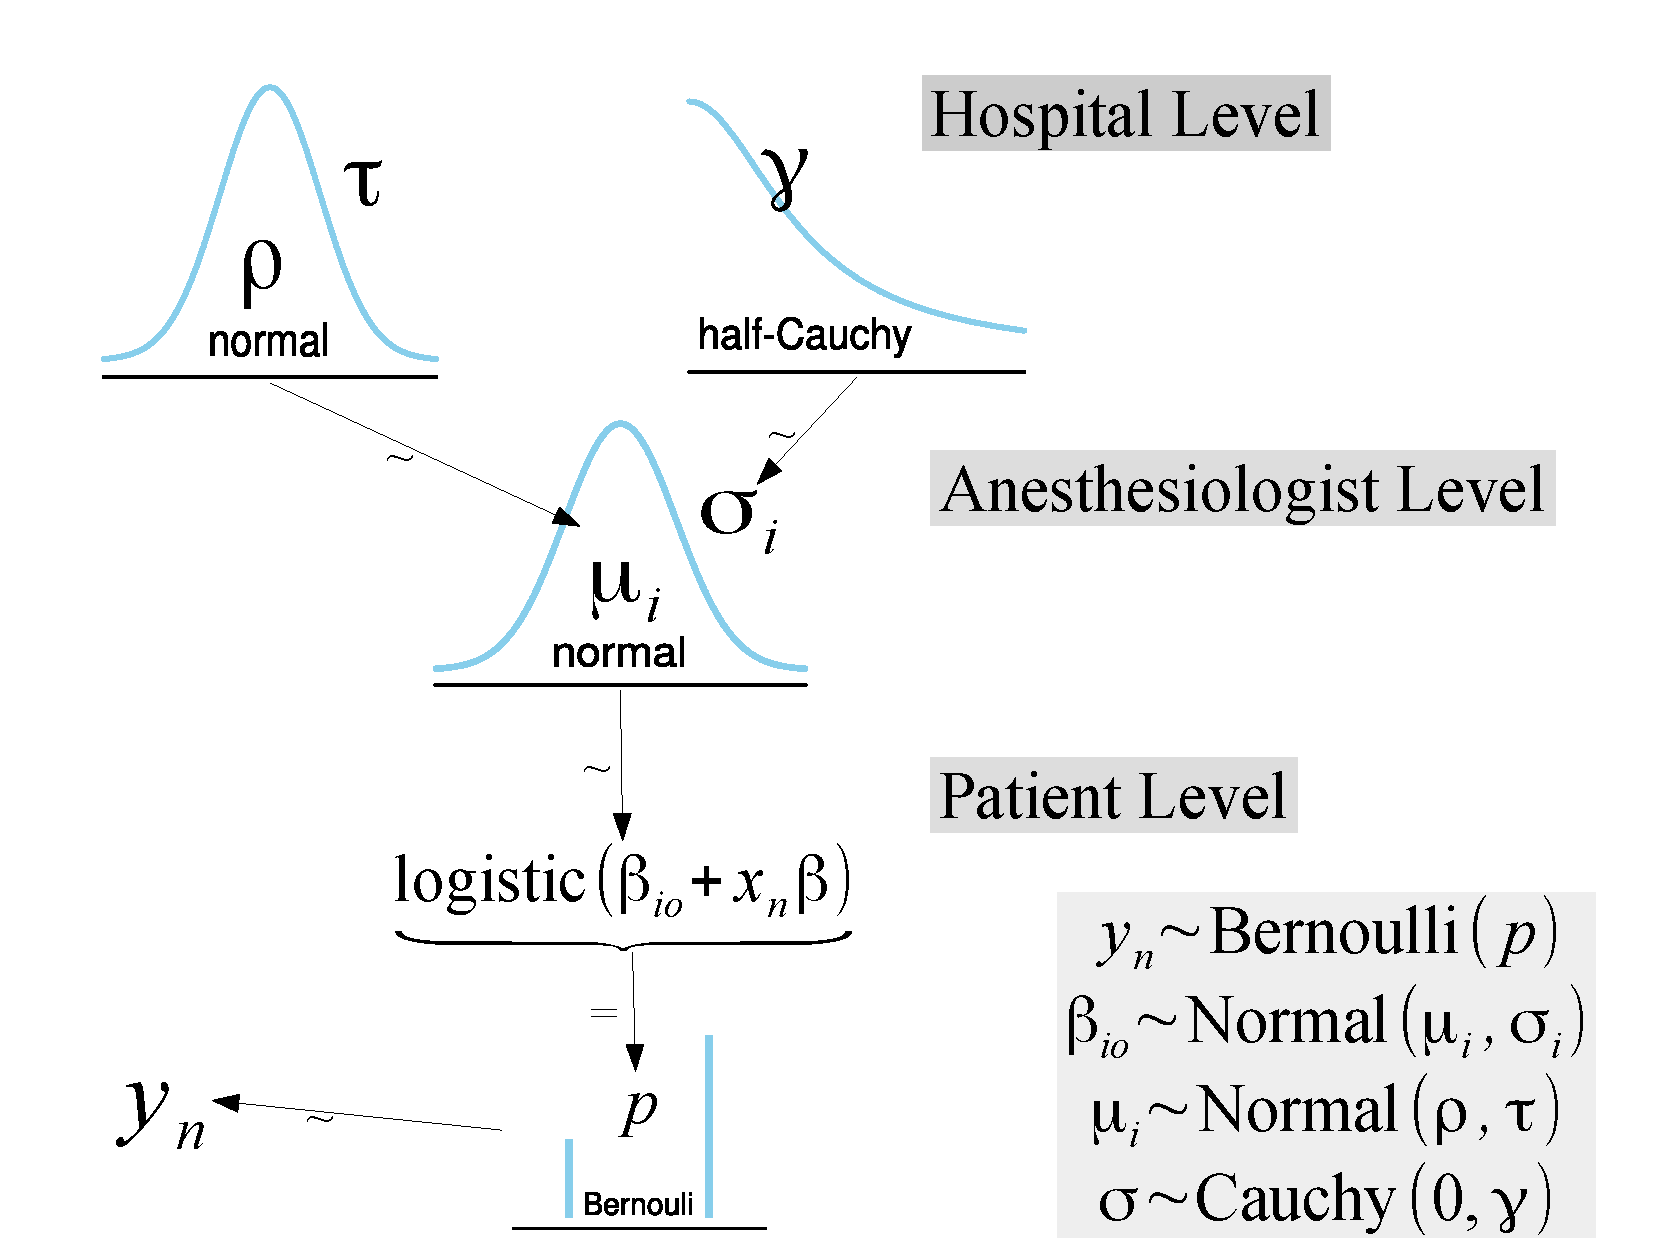
\includegraphics[width=0.4\textwidth]{Figures/DistrogramNACOR.pdf} 
\caption{Hierarchical structure of health care delivered in the perioperative setting.}
\label{fig:NACOR}
\end{wrapfigure}

Figure \ref{fig:NACOR} illustrates the hierarchical structure of health care delivery with our model on anesthesia quality with data from the National Anesthesia Outcomes Registry . The (dichotomous) outcome of particular anesthetic for a given individual will depend on the surgical procedure the patient is undergoing and under which service, but also on the local institutional culture and indeed the individual anesthesia provider and his or her qualifications and preferences\cite{AndreaeWhite2015}; Outcome $y_n$ for the $n^{th}$ patient is a Boolean indicator predicted by a logistic regression. We allow the patient intercept $\beta_{oi}$ to vary according to the $i^{th}$ anesthesiology provider caring for the patient. The provider level mean $\mu_i$ and within-provider variance $\sigma_i$ are modeled to vary by hospital. $x_n$ is a vector of patient level predictors, $\beta$ is a vector of regression coefficients.  

We seek to further substantiate the nested structure of outcome data in health care with two examples from labor analgesia and spine surgery: Anesthesiologists may feel more or less inclined or competent to offer regional anesthesia techniques; provision of epidural labor anesthesia varies widely across the nation and within an institution and is predicted by socioeconomic and racial patient characteristics \cite{Rust2004,Glance2007}. Bleeding during spine surgery is substantially less, if performed by a neurosurgeons versus by an orthopedic surgeon; while true on average, an individual gifted orthopedic surgeon may outperform the average neurosurgeon with regards to surgical blood loss.

\section*{Hierarchical models capture contemporary health care practice realistically}
Hierarchical modeling could transform electronic health records based outcomes research, because the evident rich spatial and temporal organization of electronic health records is most realistically captured in multilevel hierarchical statistical models. However, efficient model fit and computational implementation are still difficult.  Additional depth of data (simply more units of observation) would increase power and make our clinical data analysis easier. Rather, there is more breadth to the data: more subgroups, locations, provider or time granularity than is currently being modeled, more partial, incomplete and noisy measurements that cannot easily be incorporated into standard models, more related studies available for meta-analysis\cite{Andreae2015,Andreae2012}.

\subsection*{Modeling the multifaceted correlations in EHR is reflecting actual clinical practice}
To realistically model the multifaceted correlations seen in actual clinical practice, when we fitted a regression model to investigate predictors of anesthesia quality in the NACOR database, we wanted regression coefficients to vary by provider, providers again nested by service or by hospital\cite{AndreaeWhite2015}. We needed to control for the surgical procedure type as a random effect as well, with thousands of different surgical procedures performed in the NACOR population. The number of parameters to estimate grows very quickly and so do the potential interactions. Even with very large data sets, the sample size in each subgroup will shrink rapidly; estimates using least squares or maximum likelihood will become noisy and thus often become essentially useless. One solution lies in hierarchical modeling, where we estimate hyper-parameters and hyper-hyper-parameters (Figure~ \ref{fig:NACOR}), to represent how lower level parameters vary across different groupings \cite{Bafumi_Gelman_2007}. In hierarchical models, we take advantage of shrinkage, in other words we can borrow strength from larger samples to improve estimates for smaller subgroups as explained below \cite{ParkGelman2004bayesian}.

\subsection*{Hierarchical models provide efficient inferences with partial pooling}
Inference based on partial pooling outperforms (a) the No-pooling and (b) the complete-pooling approaches, as can be shown mathematically \cite{Efron_1975} or via cross-validation \cite{Gelman-Hill_2014}.  

\begin{itemize}

\item (a) Using the No-pooling approach, we would estimate the model for each specific subset of interest separately. But this leads to far too many sub-classifications, e.g. one model for each type of surgery, thus too small samples in any given subgroup for useful inferences, if we fully explore the complexity and granularity, the richness of the EMR data. 
\item (b) Employing complete pooling or structural modeling constitutes the other extreme of the spectrum, but the implied hard constraints on the coefficients in different groups may lead to bias, negating the obvious known differences in the data, for example between patients undergoing tracheotomy versus cesarean section: we gloss over such detail and lose granularity. 
\end{itemize}

We choose the middle ground: for our richly organized NACOR data set, inference using partial pooling or hierarchical modeling is especially effective , because the estimate of each individual parameter is simultaneously informed by data from all the other patients in our cohort, improving inferences in particular for subgroups with sparse data. \cite{Gelman2009}. Efron explained this apparent paradox well to non-statisticians in the \href{http://www.nature.com/scientificamerican/journal/v236/n5/pdf/scientificamerican0577-119.pdf}{Scientific American} \cite{Stein_paradox_Scientific_American}. Our co-investigator Dr. Hall applied this recently to seizure prediction \cite{Hall2009a}. 

\section*{Meta-analysis: hierarchical modeling for data driven outcomes research}
Meta-analysis, the synthesis of clinical outcome data to support evidence based decision making, is another example of hierarchical modeling, where current software and classical modeling approaches limit progress in data driven outcomes research \cite{Andreae2015} Clinicians are familiar with systematic reviews and meta-analysis\cite{Sackett1996}. Evidence synthesis (a more accurate term than meta-analysis) is a powerful tool to pool clinical trials to guide evidence based clinical care \cite{Ashby2000}. Rigorous evidence synthesis is considered the highest level of evidence to support clinical decision making \cite{Cook1997}. 

\subsection*{Variance in study design and outcome reporting hamper evidence synthesis}
However, studies on perioperative outcomes tend to vary in design and reported outcomes\cite{Andreae2013}, making evidence synthesis challenging with classical or frequentist statistical models\cite{Spiegelhalter_11134920}, (see letter of support by Dr. Sacks). Different study designs can make it difficult to perform meta-analysis or meta-regression with classical methods and standard systematic review software \cite{Deeks2011chapter}. Classical meta-analysis may also underestimate the between-study-variability for small numbers of trials\cite{Song2012,Cornell2014,Andreae2015}. \textit{Classical} meta-analysis is an example of data with a \textit{single} level of hierarchical grouping: patients' outcomes are grouped within clinical trials \cite{egger2008systematic}. There are however several constraints and limitations with this classical approach to meta-analysis, which can be overcome with more sophisticated hierarchical modeling  \cite{Andreae2015,Thompson2002,Abroug2011}. 

\subsubsection*{Hierarchical models to integrate all available data for evidence synthesis}

\begin{wrapfigure}{l}{0.4\textwidth} 
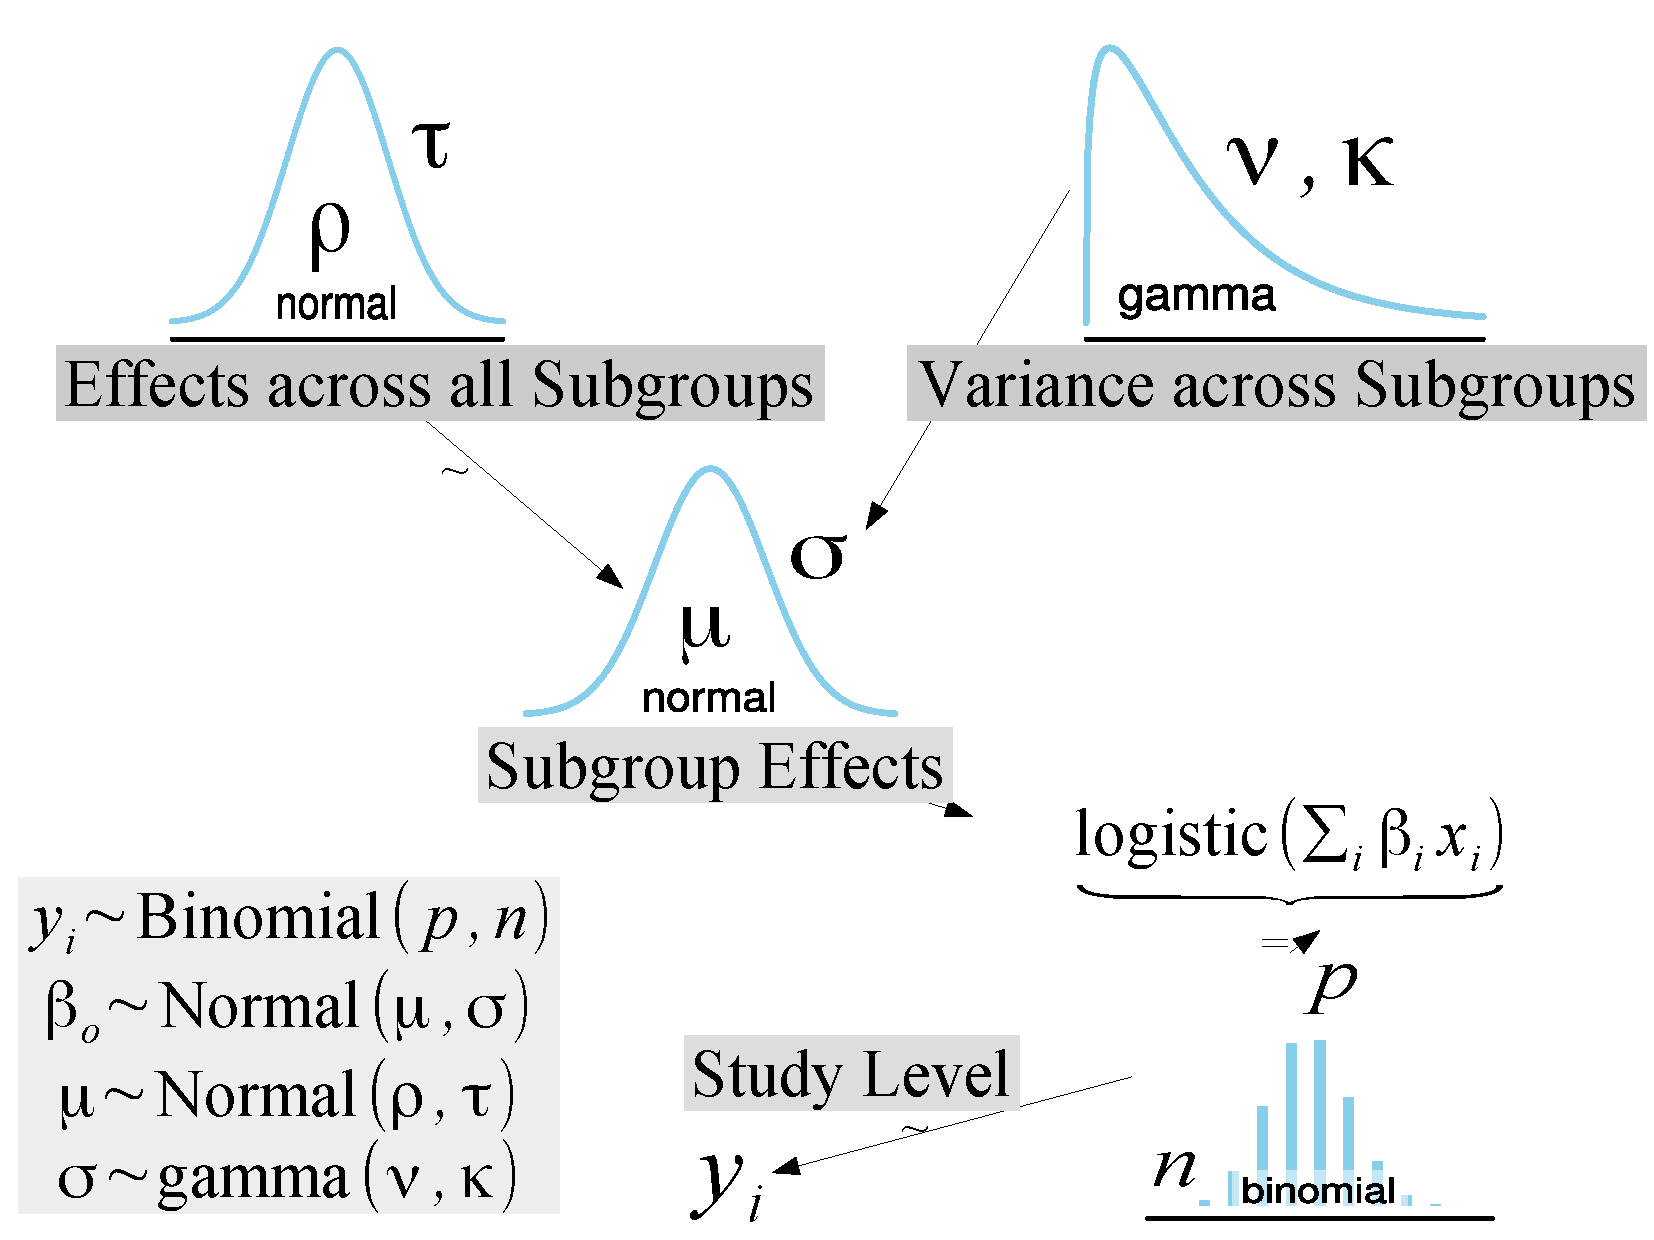
\includegraphics[width=0.4\textwidth]{Figures/DistrogramMetaAnalysis.pdf} 
\caption{\footnotesize Simplified distrogram to illustrate multi-level meta-analysis.}
\label{fig:MetaAnalysis}
\end{wrapfigure}

Trial or population characteristics may introduce another level of grouping, for example pooling long term outcomes after regional anesthesia by surgical intervention \cite{Andreae2013,Abroug2011}. Trials may observe outcomes at several sequential follow-up visit, leading to repeated (correlated) observations grouped by patient, (which are then grouped by trial in the  meta-analysis).  We build a multilevel hierarchical model to pool individual patient data with continuous and dichotomous aggregate study level data, clustered at the study level by followup interval and at the study level by surgical intervention performed (Figure \ref{fig:MetaAnalysis}). Besides the three levels of hierarchical modeling just outlined (follow-up observations grouped by patient, patients grouped withing trials, trials within population), additional groupings or hierarchical levels concern exposure dose, as meta-regression of effect dose dependence may explain substantial between-study variance in outcomes reported to reconcile study findings \cite{Andreae2015}. Evidence synthesis may seek to integrate continuous with dichotomous outcome measures \cite{AndreaeJohnsonAbstract2013}, because to be valid meta-analysis must integrate \textit{all} available data sources \cite{Deeks2011chapter}. However, short of having access to all individual patient data, the integration of dichotomous outcomes with continuous outcomes is challenging with classical methods\cite{Andreae2015}, especially as often insufficient aggregate results are reported \cite{Roth2015CriticalCare}. 

\subsection*{The antithesis of complete versus no-pooling limits meta-analysis of perioperative outcomes}
To illuminate how the antimony between complete versus non-pooling also limits evidence synthesis, we consider meta-analysis of trials with repeated observations of the outcome of interest. The follow-up intervals at which perioperative outcomes are reported often vary in different studies. What is more, some studies report repeated measures, others only a single terminal observation; This leads to the same issue of (a) complete pooling versus (b) No-pooling also in evidence synthesis \cite{Roth2015CriticalCare}.

\begin{itemize}
\item (b) No-pooling: 
Conducting meta-analyses at each time point, i.e. performing separate meta-analysis for each follow-up visit separately, would drastically reduce sample size and hence power and precision, undermining the main strength of meta-analysis.
\item (a) Complete pooling:
Evidence synthesis irrespective of follow-up-time, i.e. of all effect estimates at different time points, fails to consider the correlation of repeated measure and is only appropriate if the effect estimates does not depend on how long after the intervention the outcome was observed. This is obviously often an untenable assumption.
\end{itemize}

\subsubsection*{Clustering and correlations can bias clinical inferences in meta-analysis }
In addition to a possible influence on the point estimate of the measure of effect, an even more concerning bias results from failing to consider correlations between outcomes. A significant effect can be transformed into a non-significant effect (or vice versa), changing the confidence interval of the pooled effect estimate, be over- or underestimating the variability of correlated outcomes. For example assume an estimated overall relative risk (RR) of 0.8 for an intervention across all studies pooled. The estimation of a 95\% confidence interval of 0.55-1.15 would lead to the inference of "no statistically significant effect" and thwart further attempt to study this intervention, while a 95\% confidence interval of 0.7-0.9 for the effect estimate may lead to widespread adoption of this therapeutic approach. Interpretation of meta-analyses, and especially Cochrane Reviews, in clinical practice are unfortunately often reduced to "shows a significant effect" vs. "shows no significant effect". Incorrect inferences can have huge clinical impact.

\subsubsection*{Ecological, disease and geographic study level characteristics can influence inferences}
Besides clustering by reported time endpoint, there are other forms of ecological bias or clusters to be considered in meta-analysis; certain geographical or historical settings, similar surgical procedures or diseases will lead to correlated outcomes in patient cohorts \cite{Abroug2011,Andreae2013,Andreae2015,Roth2015CriticalCare}. Therefore, the same antimony of complete pooling versus no-pooling limits meta-analysis for perioperative outcomes and hinders evidence based medicine. Besides the effects estimates themselves, their precision, inter and within study variability may differ considerably contingent on disease, procedure or other study level characteristics \cite{Andreae2013,Andreae2015,Roth2015CriticalCare}.

\subsubsection*{Partial pooling across distinct, but similar populations}
The principle  of clustered and hierarchical modeling for evidence synthesis is analogous to outcome research in general, when we consider effects more prominent in one trial or subgroup of the populations and not as strong in another similar but distinct trial or subgroup. An example of this would be the meta-analyses of a treatment effect in conditions with different but related etiologies, for example the spectrum of HIV-related, idiopathic, diabetic, and traumatic chronic painful neuropathy \cite{Andreae2015}. Information in one subset or study population can and should inform estimates in other similar populations at least to some extend in a hierarchical meta-analysis. The principle applies in other fields of medicine, e.g. critical care as well \cite{Roth2015CriticalCare} and becomes more relevant if average effect sizes, precision of effect estimates, inter- and within-subgroup variability differ considerably from the subgroups used to obtain aforementioned findings.

\subsection*{Hierarchical modeling improves data driven outcomes research in our contemporary hierarchically structured health care system}
 
Multi-level hierarchical models may hence be a useful tool to analyses heterogeneous perioperative outcome data. This is true for meta-analysis of long-term studies with varied design to better inform clinical decisions\cite{AndreaeJohnsonAbstract2013,Spiegelhalter2004bayesian} and for data driven outcomes research  in our hierarchically structured contemporary health care delivery system. Complex multilevel models can be difficult to fit with standard software and should be more accessible, (see letter of support by Drs. OMalley).

\subsection*{Clustering can bias estimation of confidence intervals.} To correctly estimate confidence intervals even in a simple Student t-test, we have to take into account if the data are observed in the same patient repeatedly, i.e. if they are clustered and correlated. Failure to take into account correlations in clustered observation may lead to incorrect inferences. Based on the empirical (robust) (weighted jackknife) methods, the confidence intervals are correct, but such approaches are often ignored in EHR research and they depend on convergence characteristics that may not hold in faceted EHR data. 

\section*{Integrating incomplete data into clustered EHR modeling}

Too often data scientists either (1) fit complex model but limit the analysis to complete cases, ignoring the missing or incomplete data or (2) impute the missing data, but build overly simplified models of the scientific question of interest, to limit complexity of the overall model, (see letter of support by Dr. Mirhaji). More accessible hierarchical modeling could better integrate the two elements. Missing predictors are imputed on a lower level of the model. The imputed missing data point with its confidence interval (indicating the precision of the imputation) is then fed into the estimation at the next higher level of the model \cite{Gelman2001imputation}. 

\subsection*{EHR data are not missing at random.} Physicians chose which test to get to inform specific therapeutic decisions and different types of data are recorded in different clinical setting, e.g. arterial lines may not be permissible on the floor, vitals are recorded in greater detail and more frequently in high dependency units like the ICU. 

\section*{Difficulty to fit and explore complex hierarchical models}
In approach we explain  how taking both missing data imputation and clustering can be integrated into a single model. This challenge is currently compounded the dearth of tools to explore the enormous data stream generated in Markov chain Monte Carlo (MCMC) simulations to explore and trouble shoot fitted hierarchical models.  

\subsection*{Punchline: Hierarchical models  are best suited to reflect the clustered structure of contemporary health care delivery realistically.}

\part*{Innovation}

We propose to build two software packages. \textit{rstanarm} to make multi-level hierarchical modeling more accessible and \textit{shinystan} for graphical exploration and confirmation. \textit{rstanarm} and \textit{shinystan} will address the dearth of accessible software to build complex multilevel hierarchical models, assess and troubleshoot model convergence, confirm congruence of model and data and improve statistical inference, (see letter of support by Dr. DiMaggio). In the process, we will advance statistical methods and algorithms for convergence diagnostics and integrate missing data imputation with advanced hierarchical modeling in a single software package.  

\subsection*{Accessible advanced hierarchical modeling for EHR}

For \textit{basic} hierarchical models, there are simple and accessible software package both in the frequentistist and the Bayesian paradigm, but multilevel hierarchical modeling is currently restricted to data scientists and statisticians with advanced computational and statistical expertise. Even for these specialists, the step learning curve of advanced probabilistic programming languages like \textit{Stan} constitutes a significant barrier to harness the full potential of hierarchical modeling for data driven outcomes research (see letter of support by Drs. Sacks and OMalley).

\textit{rstanarm} is the first accessible, yet ultra-fast and flexible package to allow even very advanced hierarchical modeling for large data sets based on very simple familiar model specification. It is open source, and free to the public. The tranparent modeling approach in \textit{rstanarm} will make analysis more reproducible and reliable enough even for federal regulatory processes. 

\subsection*{Fast and flexible hierarchical modeling for realistic data driven outcomes research }

\begin{wrapfigure}{l}{.3\textwidth}
  \vspace{-15pt}
 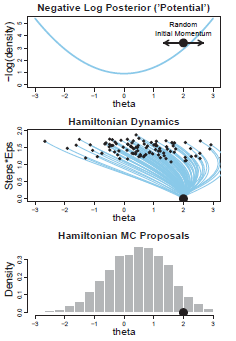
\includegraphics[scale=0.85]{Figures/Hamiltonian.png}
  \vspace{-20pt}
  \caption{Hamiltonian MCMC}
    \label{fig:Hamiltonian}
 \vspace{- 30 pt}
\end{wrapfigure}

Our \textit{rstanarm} is based on the Hamiltonian Monte Carlo algorithm implemented in Stan, which is orders of magnitude faster than existing MCMC algorithms. Figure \ref{fig:Hamiltonian} reproduces Fig 14 in Kruschke \cite{Kruschke_Book_2014} to illustrate how \textit{Stan's} Hamiltonian algorithm achieves faster convergence by using momentum to optimize the next proposal. The current proposal's higher momentum (black dot) is indicated in the top panel. The middle panel illustrates how their momentum steers random samples to the mode of the posterior distribution (shown in lower panel), accelerating convergence. 

This matters as the sequential process of fitting complex multilevel models for Big Data  and testing them can be cumbersome and slow even for the initiated and sophisticated data scientists who are able to writing complex code to implement them. Multilevel hierarchical models can compromise transparency with lengthy complicated programming code, making the process error prone (see letter of support by Dr. Pace). Typically scientists have to explore and compare different angles and approaches to modeling large electronic data sets. Typically researchers need to update and tweak the model to make it more and more complex, to fit the data better or to facilitate convergence of the algorithm. With existing software, like OpenBugs or \textit{JAGS} building and updating hierarchical models sequentially for large data sets becomes prohibitively expensive in computer resources or too slow to be feasible. The challenges of fast and flexible computational implementation such limit the model sophistication (see letter by Dr. Kheterpal and Dutton). Researchers cannot fit multilevel models which reflect the actual hierarchical structure of clinical care delivered, (see letter by Dr. Sacks). \textit{rstanarm's} simple yet flexible function calls facilitate dynamic model building and updating, and allows the fitting and testing of complex models even for larger datasets. \textit{rstanarm} allows researchers to fit the model they believe to best reflect the clinical question they are investigating with EHR.

\subsection*{Improve tools for graphical exploration of hierarchical models and MCMC output}

\begin{wrapfigure}{l}{.6\textwidth}
  \vspace{-10pt}
 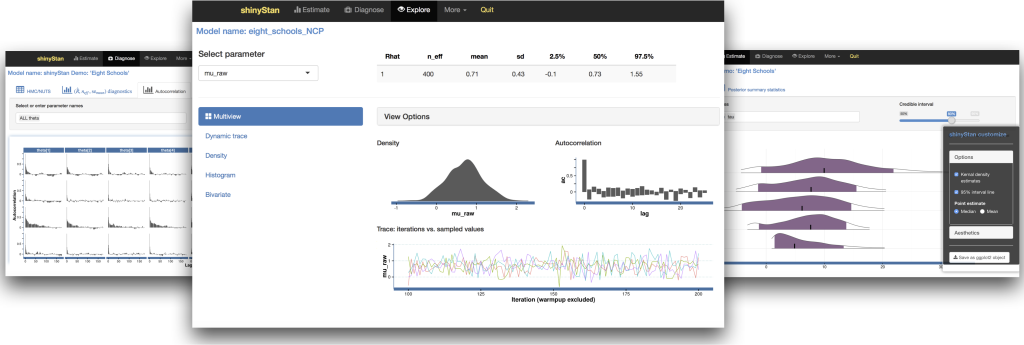
\includegraphics[scale=1.2]{Figures/shinystan.png}
  \vspace{-10pt}
  \caption{\textit{shinystan} interface}
    \label{fig:shinystan}
 \vspace{- 10pt}
\end{wrapfigure}

Accessible tools and utilities, new visual methods to explore sophisticated model and
their output would accelerate the model development, reduce modeling errors and 
fascinates inferential reasoning. \textit{shinystan} will fill in the void where 
there is currently a dearth of conceptual approaches, tools and utilities to 
analyze the very large data generated with Marcov Monte Carlo simulations 
themselves. The interactive user interface \ref{fig:shinystan} of \textit{shinystan} 
will provide powerful and easily accessible tools for posterior predictive checks 
to improve congruence of the fitted model with observed data. Advanced, refined 
and accessible model convergence diagnostics enhance model building. If a complex 
model fails to converge, knowing why is crucial to troubleshooting. \textit{shinystan} 
is already unmatched in combining ease of interactive graphical exploration 
with sophisticated graphical rendering to explore visually and parameter 
specific co-linearity, auto correlation, tree depth of Hamiltonian Monte 
Carlo algorithms and many other convergence diagnostics. We will not only 
further develop \textit{shinystan} to make it more robust, scale it to work 
faster also for larger data sets; beyond, we will develop novel graphical 
methods to assess model convergence and define and refined algorithms to 
troubleshoot model convergence with a special focus on multilevel hierarchical 
modeling. 

 

\subsection*{Heterogeneous and incomplete clinical data may limit prediction and implementation.}
Variables with strong predictive power in our model may not be recorded in all patients 
or may be missing for the time window needed for prediction, a critical limitation 
in the development of prediction algorithms and implementation of the 
therapeutic interventions (see letter of support by Dr. Mirhaji). 
Yet, incomplete data are the hallmark of EMRs. 
Likelihood-based mixed effects models for incomplete data give valid estimates 
\textit{if and only if } the data are ignorably missing; that is, the parameters 
for the missing data process are distinct from those of the main model for the 
outcome, and the data are missing at random (MAR) or Missing Completely At Random 
(MCAR), a rare condition \cite{Rubin1976}. Indeed, this is an unreasonable assumption 
for EMRs; in our example, only significant patients respiratory co-morbidity and 
symptoms will prompt physicians to request arterial blood gases (ABG). Trying to 
impute missing ABG data using multiple imputation would  hence lead to biased 
imputations as the ABG data will not be missing at random. Imputation using 
auxiliary data can overcome this limitation, as outlined below.

\subsection*{Auxiliary data can be used to impute incomplete medical records.} 

\begin{wrapfigure}{l}{10cm} 
 \vspace{-10pt}
 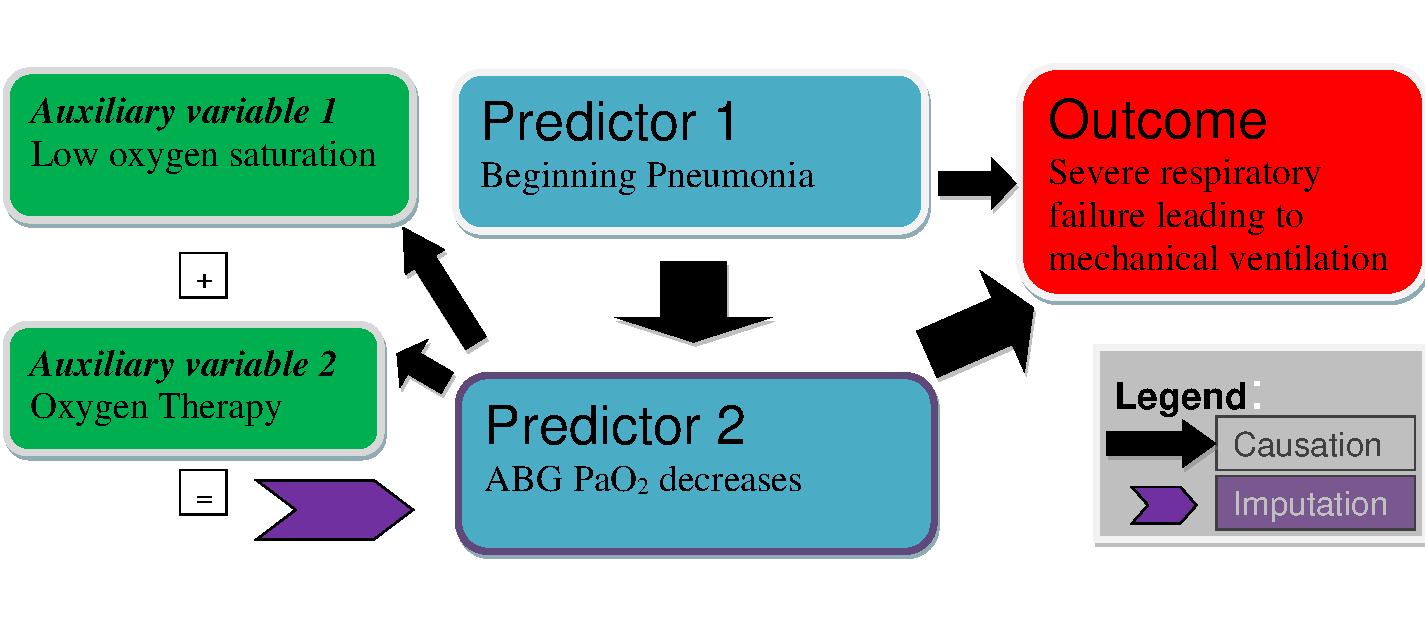
\includegraphics[scale=0.4]{Figures/Bayesian_imputation.pdf}
    \vspace{-15pt}
  \caption{Auxilliary data to impute missing information}
   \vspace{-5pt}
   \label{fig:Imputation_fig}
\end{wrapfigure}

Auxiliary data are additional information available in the form of variables known 
to be correlated with the missing data of interest 
\cite{Hall_25389642,Daniels24571539}. Figure \ref{fig:Imputation_fig} 
illustrates how we can impute incomplete data from auxiliary information 
\cite{Ibrahim2001auxilliaryImputaton,Schomaker23873614}. We know pneumonia 
impairs oxygenation, by causing respiratory failure, for example. If 
arterial $PaO_2$ (oxygen tension) is missing because arterial blood 
gases (ABG) have not been obtained, we can impute the incomplete data 
from oxygen therapy and/or peripheral oxygen saturation\cite{Hall_25389642}. 
This approach avoids the perils associated with missing at random (MAR) 
assumptions, when fitting a non-ignorable missingness model \cite{Wang_20029935}. 
Adding auxiliary variables not included in the main model for multiple imputation, 
in other words using additional information that is correlated with the missing 
outcome is an emerging approach to help correct bias 
\cite{Meng1994, Collins_11778676, Rubin1996}, often relying on 
Bayesian methods \cite{Daniels2008, Schafer1997}; joint hierarchical 
modeling, including auxiliary data to impute incomplete patient records, 
will improve the prediction model and facilitate the implementation of the 
prediction algorithm \cite{Hall_25389642}. Using auxilliary data to complete 
missing information is novel in data driven outcomes research and our 
software \textit{rstanarm} will disseminate this promising approach by 
facilitation its implementing. 

\part*{Approach}

We propose to develop two accessible software packages, (\textit{rstanarm} 
and \textit{shinystan}), for the programming language and software environment 
\textit{R} to integrate incomplete information with hierarchical modeling for 
data driven outcomes research. These software products will make multidimensional statistical and computational methods for analyzing, inspecting, displaying, 
representing, parsing, and searching high-dimensional data more accessible to 
data scientists. We will also promote and disseminate these more complex 
hierarchical modeling approaches through presentations, graduate teaching, 
workshops, online tutorials, books, YouTube videos and other publications.

We will develop our two prototypes (1) \textit{rstanarm} and (2) 
\textit{shinystan} further into solid, reliable, tested software packages. 
Both packages will serve as appendage to the $rstan$ package (we developed), 
which enables the most common applied regression models to be estimated using 
novel Hamiltonian Monte Carlo algorithms. We will makes our new two 
packages \textit{rstanarm} and \textit{shinystan} available to researchers 
and the general public via the free software repository CRAN. 

This project (software development and dissemination) will be guided by 
our multidisciplinary project team. The team will conduct its work through 
regularly scheduled weekly meetings, and continued online collaboration via 
Github, Google hangout and email. 



\section*{Preliminary work}

\subsection*{Prior work in statistical software development and data driven outcomes research} Dr. Andreae published several meta-analyses and synthesized the evidence 
from clinical trials by pooling aggregate and individual patient data, when 
published results were insufficient for classical meta-analysis 
\cite{AndreaeJohnsonAbstract2013, Andreae2013, Andreae2015, Carter2015, Atchabahian2015}. Dr. Andreae, Hall, Goodrich and collaborators used the software 
prototype \textit{rstanarm} and \textit{shinystan} to build a multilevel 
hierarchical model to investigate health care disparities and quality of 
anesthesia delivery in the large National Clinical Outcomes Registry maintained 
by the American Society of Anesthesiology \cite{AndreaeWhite2015}. Dr. Goodrich 
build \textit{mi}, a software package for the programming language and 
software environment R to impute missing data \cite{miCRAN}. Drs. Goodrich 
and Gelman together developed other several widely cited and used software packages including the probabilistic programming language Stan\cite{Stan_Software_2014}, 
the basis for the proposed work. Dr. Hall also published on missing data 
imputation \cite{Hall2009a, Wang_20029935, Wang_20029935} and is nationally 
recognized for the development and application of change point models in 
epidemiology and surveillance 
\cite{Hall2000, Hall2001, Hall2003bayesian, Hall2009, Hall2015}. 
More recently, Dr. Hall played a major role as the lead statistician 
for the World Trade Center (WTC) Health Program at the Fire Department 
of the City of New York, supervising data analyses based on medical 
records \cite{Aldrich2010, Hall2015, Zeig-Owens2011}.  
Dr. Gong's ongoing NIH funded trial to predict and improve 
respiratory outcomes after intubation based on real time 
electronic medical records is just one of many examples of her 
leading role in applied data driven outcomes research 
\cite{Gong2005, Gong2010, Gajic2011, Yu_24970344, Kor2014}. 
Dr. Gelman is internationally recognized as a leader in Bayesian and hierarchical 
modeling and data imputation 
\cite{Gelman1998notasked, Gelman2001imputation, Hoffman2014, Gelman-Hill_2014}. 
Dr. Gelman, co-investigator on this grant, and his collaborators has been laying the 
theoretical ground work for the development of the ultra-fast Hamiltonian 
Monte Carlo algorithms \cite{Hoffman2014,Stan_Software_2014} 
that are at the basis of \textit{Stan}, the engine 
under the hood of our user oriented software package \textit{rstanarm}, 
this project proposes to develop. His team includes Dr. Betancourt, 
consultant on this grant with his special expertise on the differential 
geometry of the underlying Hamiltonian Monte Carlo algorithm
motivating automated tuning heuristics and certain optimality criteria 
\cite{BetancourtGeometry2016}, which will play a 
critical part in our programming of the \textit{Stan} model library 
which \textit{rstanarm} will call on and in the tools for graphical exploration
we propose to implement in \textit{shinystan}.

\subsection*{The trajectory leading to the development of the prototype software} 

\begin{wrapfigure}{l}{0.6\textwidth} %this figure will be at the right
    \centering
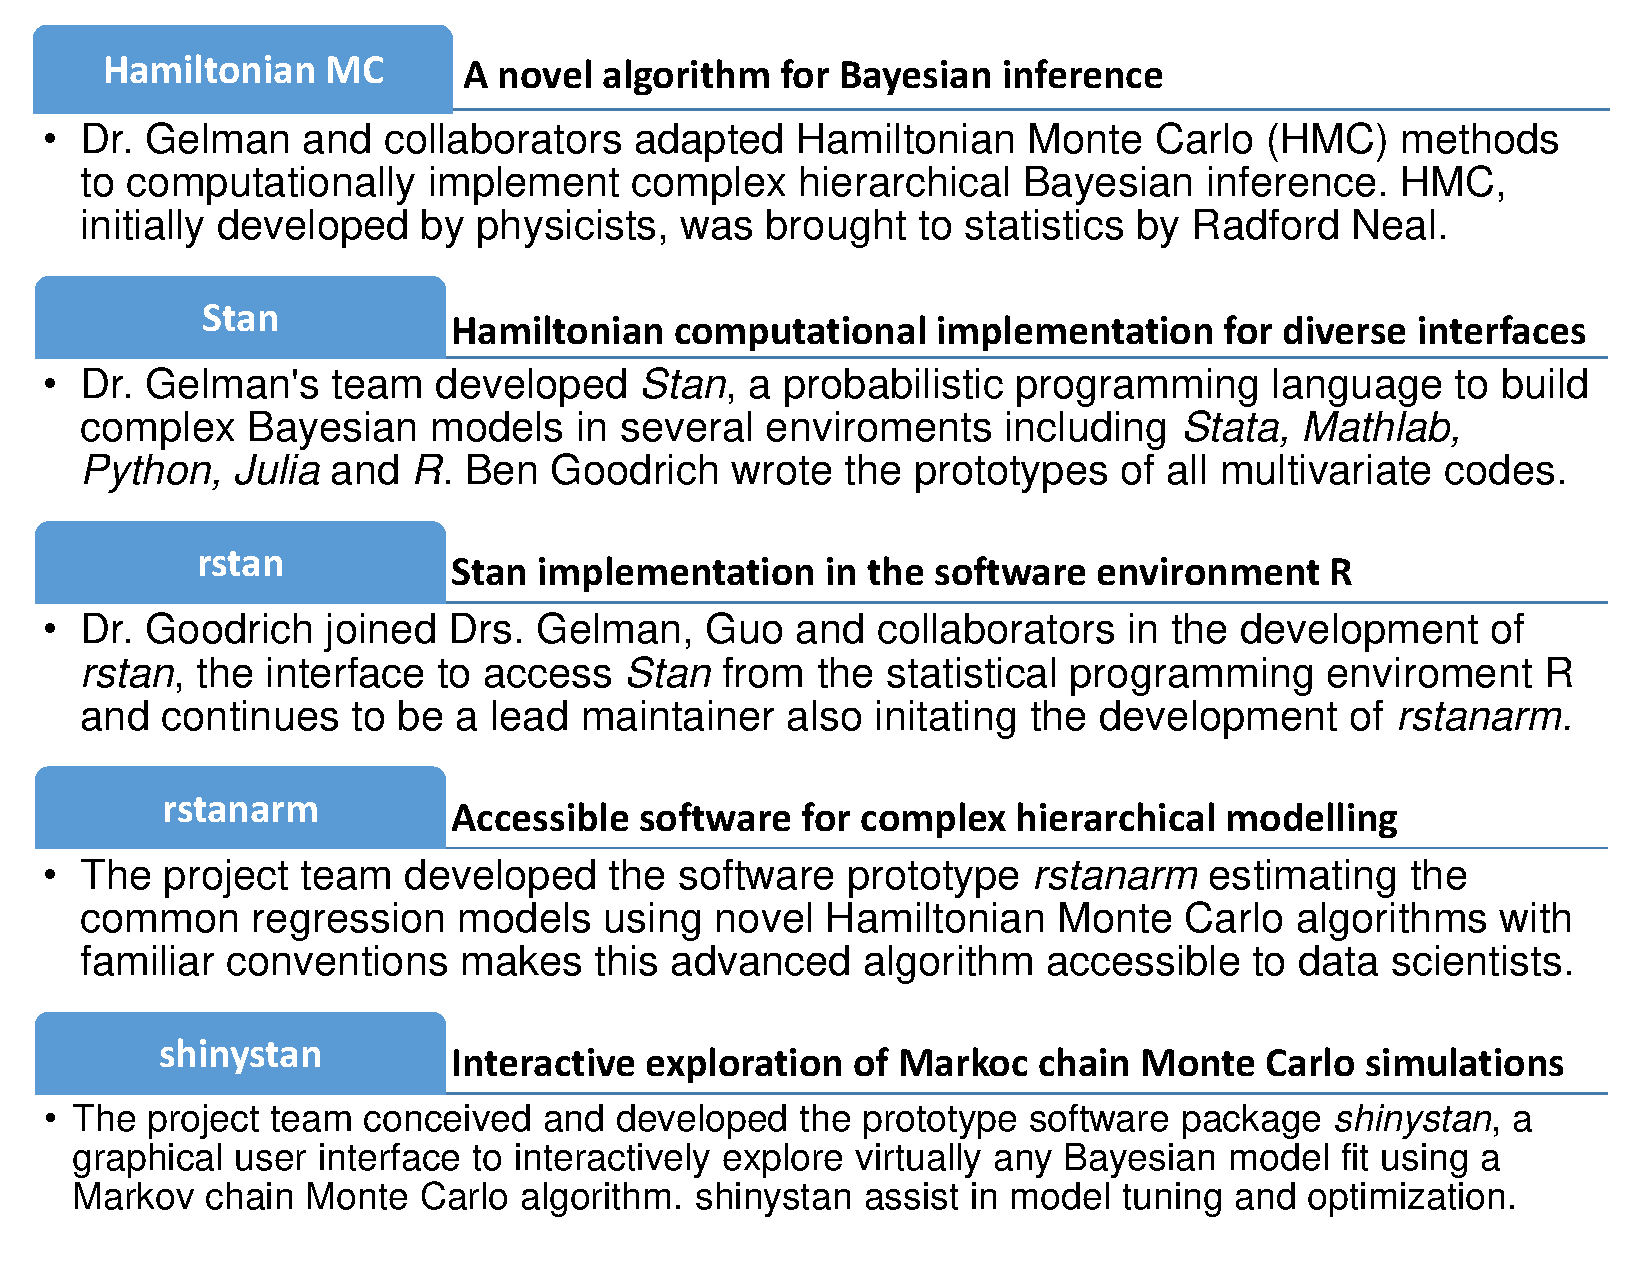
\includegraphics[width=0.6\textwidth]{Figures/SoftwareTrajectory.pdf}
\end{wrapfigure}

Dr. Goodrich and Andreae and their collaborators worked together on the preliminary software packages \textit{shinystan} and \textit{rstanarm}, which are appendages and developments based on the \textit{rstan} package that enables some of the most common applied regression models to be estimated using Markov Chain Monte Carlo. The National Institute of Health, the Center for Disease Control and the National Science Foundation, (NIH: 5R01GM074806, 5KL2TR001071, UH2-HL125119,  CDC: U01 OH010711-01 and NSF: SES-1205516) funded much of our team's prior related algorithms and model and software development and their application to complex biomedical data driven outcomes research. The proposed work is hence a direct continuation of the above described preliminary work of developing and implementing novel ground breaking algorithms for hierarchical modeling of complex data and their biomedical applications. In the graphic to the left above, we outline the trajectory that led to the current project proposal.


\section*{Project scope and goals }

The project proposes to develop two accessible software packages for the programming language and software environment \textit{R} to integrate incomplete information with hierarchical modeling for data driven outcomes research. We propose to develop two applications.

\subsection*{rstanarm for accessible multilevel hierarchical modeling}
The first proposed software package \textit{rstanarm} should allow data scientists to build the most common applied regression models and multi-level hierarchical models based on the ultra-fast Hamiltonian Monte Carlo (HMC) algorithm implemented in \textit{Stan} without (a) the need to understand the underlying complexities (e.g. auxiliary parameterization) normally required to optimize convergence and without (b) the need to build complex contrast matrices  or keep track of level indexing. Using the same familiar notation for model formulation as other popular software packages for linear and mixed modeling in R/Rstudio like \textit{lme4} \cite{lme4}, will make model building easy for novice \textit{rstanarm} users. 

\subsection*{shinystan for interactive graphical exploration and diagnosis of MCMC simulations}  
The second package, \textit{shinystan}, is a graphical user interface for interactively exploring virtually any model fit using any Markov chain Monte Carlo (MCMC) algorithm. As a package for R/Rstudio, shinystan  provides multidimensional statistical, graphical and computational tools for any analyzing, inspecting, displaying, representing, parsing, and searching high-dimensional MCMC output, but is optimized for HMC. By using a web-based interactive intuitive user interface \textit{shinystan} is user-friendly and requires minimal training for novices.

\subsection*{rstanarm and shinystan prototypes are available on the \textit{R} software repository CRAN}
We build prototypes for both software packages \textit{rstanarm} \cite{rstanarm} and \textit{shinystan} \cite{shinystan, Team2015}, available on the \textit{R} software repository CRAN. The project proposes to further develop these two prototypes \textit{rstanarm} and \textit{shinystan} into solid, reliable, tested R packages and to disseminate their use. Both packages will serve as appendage to the \textit{rstan} package (we developed), which enables the most common applied regression models to be estimated using novel Hamiltonian Monte Carlo algorithms. The final product packages will be available to researchers and the general public via the free software repository CRAN. 

Estimates pre-compiled regression models using the 'rstan' package, which provides
the R interface to the Stan C++ library for Bayesian estimation. Users specify models via the customary R syntax with a formula and data.frame plus some additional arguments for priors.

\section*{Software Specification}

\subsection*{rstanarm}
The software package \href{https://github.com/stan-dev/rstanarm}{\textit{rstanarm}}
will enable the estimation of advanced applied general linear regression models using 
the existing probabilistic programming language \textit{Stan}. 
\textit{rstanarm} implements full Bayesian statistical inference;  
however, \textit{rstanarm} will allow users to specify their complex 
hierarchical models relying on the simplified syntax already commonly 
used in standard software packages like \textit{lme4} in the statistical 
software environment \textit{R}. 

\subsubsection*{rstanarm allows simple specification for complex hierarchical models}

Data scientists familiar with the widely used statistical software environment R will 
find \textit{rstanarm} intuitive, because models are specified using the familiar 
standard R modeling syntax to describe the mean structure of even complex models. 
For example, analogously to \textit{lme4}, \textit{rstanarm} uses a two-sided 
linear formula syntax describing both the fixed-effects and random-effects of 
a model, e.g.:

\begin{wrapfigure}{l}{.2\textwidth}
\vspace{-20pt}
\begin{equation}
y \sim x1 +(x2|x3)
\end{equation}
\vspace{-30pt}
\end{wrapfigure}

where the dependent response variable $y$ is on the left of a Tilde ($\sim$) operator; 
the independent terms, $x_1, x_2...$ are on the right and separated by the $+$ 
operator. Random-effects terms are distinguished by vertical bars $|$ 
separating expressions for design matrices from grouping factors. Clinical data 
scientist can therefore take advantage of the  more efficient inference of the 
cutting edge HMC algorithms implemented in \textit{Stan}, without knowledge of 
the underlying programming language or the auxiliary reparametrizations useful to 
achieve faster model convergence, which we discuss further below.

\subsubsection*{A suite of pre-compiled Stan models allows for a simple call to complex modeling functions}

Our prototype of \textit{rstanarm} already implements many generalized linear 
models with and without group-specific terms. We wrote many optimized models 
in the probabilistic programming language \textit{Stan}, which have been 
pre-compiled, saving time during function calls for recurrent sequential 
complex model building. Users therefore can now build complex models via simple top level 
functions, interfacing only with a wrapper function as detailed below.

\begin{wraptable}{l}{0.6\textwidth}
\footnotesize
\begin{tabular}{@{}
>{\columncolor[HTML]{EFEFEF}}l l@{}}
\toprule
\textbf{Function Call} & \textbf{Underlying process}                        \\ \midrule
stan\_aov               & User interface for simplified model specification  \\
stan\_lm               & Parsing linear model specification \\
stan\_lm.fit           & Workhorse function to call pre-comiled \textit{Stan} model  \\
lm.stan                & Pre-compiled optimized model written in \textit{Stan}                   \\ \bottomrule
\end{tabular}
\label{ProcessTable}
\end{wraptable}

For an ANOVA model for example, the wrapper function $stan\_aov$ parses the 
model specification and hands the data and user specification via a linear 
model functions, in this case $stan\_lm$ to a lower level workhorse function, 
here $stan\_lm.fit$, which in turn creates model frame and design matrix and 
calls the specific pre-compiled and optimized \textit{Stan} model function 
$lm.stan$. The latter formats and returns the Hamiltonian Markov chain Monte 
Carlo output back via the user interface function $stan\_aov$ to the data scientist.

The $stan\_lm$, $stan\_glm$ and $stan\_glmer$ functions, (accessible to the 
more advanced user) are similar in syntax to the R software functions $glm$ 
and $glmer$ as used in the R package $lme4$, respectively, but rather than 
maximum likelihood estimation of classical generalized linear models, full 
Bayesian estimation is performed via Hamiltonian Markov chain Monte Carlo 
simulations. If neutral "minimally informative" priors are chosen (AKA 
"empirical Bayesian"), this yields results very similar, if not 
identical to classical frequentist inference \cite{Gelman-Hill_2014}, making \textit{rstanarm} a very universal user-friendly software suite to estimate complex hierarchical models.

\subsubsection*{Prior specification for regularization or to incorporate external information}

Priors \textit{can} incorporate subjective beliefs or existing information 
about a parameter,  which we discussed in more detail under significance \cite{carlin1997bayes}. 
Priors can be used to regularize classical models \cite{gelman2008weakly}. 
Bayesian models require priors and the prototype of \textit{rstanarm} 
automatically adds independent weakly 
informative priors on the coefficients of the generalized linear model, 
leading to inferences similar to classical statistics,  but more informative 
prior can be specified by the user. Especially in hierarchical modeling, 
regularization with priors can help convergence and improve inferences 
\cite{Gelman-Hill_2014}. In \textit{rstanarm}, specification of the prior 
can such be left to the default implementation or the user can choose from 
a broad array of distribution, e.g. for the intercept one might choose the 
Student t distribution, which approaches the normal distribution as the 
degrees of freedom approach infinity and as the degrees of freedom are 
one, the Cauchy distribution, leaving the user the option of robust 
priors to allow for outliers to achieve more robust inference. 


\subsection*{shinystan}
We propose to develop \href{http://andrewgelman.com/2015/03/02/introducing-shinystan/}
{\textit{shinystan}} as a the graphical user interface for interactively 
exploring virtually any Bayesian model fit using a Markov chain Monte Carlo algorithm, 
but optimized for \textit{rstanarm} and \textit{Stan}. 

\subsubsection*{Goal: interactive intuitive graphical exploration of MCMC output} 
To extract the results from objects representing model fits, data scientist can 
use generic extractor functions such as print(), coef(), but often lack a suitable 
method for extracting an interesting result of the model fit and have to resort to 
writing tedious code to customize their own. Important model diagnostics 
(e.g. influence() to assess  homoscedastic residual errors) are not 
developed even for classical multi-level models \cite{Galecki2013linear}, 
and data scientists certainly lack tools for interactive intuitive graphical 
exploration of MCMC simulations.

\subsubsection*{Implementation}
We will implement \textit{shinystan} in \textit{Shiny}, an R package for interactive 
web applications. The graphical rendering of our proposed package \textit{shinystan} 
is building on the superb graphical package \textit{ggplot} by Hackley Wickham. 
Many of our new graphical functions of \textit{shinystan} will eventually be 
integrated directly into \textit{Rstan} to allow users to integrate the graphical 
and numerical output of \textit{shinystan} directly into reports generated with 
markdown in R through the \textit{knitr} package.

\subsubsection*{Model checking}
shinystan will facilitate many diagnostics to optimize model convergence, explore unexpected parameter correlations and asses the correctness of the model specification. Here we will delineate two examples.
\begin{itemize}
\item (a) residual diagnostics, e.g. for continuous covariates, a scatterplot of the residuals against the values of the covariate can also be used. Q-Q plot
 
\item (b) influence diagnostics
\end{itemize}

\subsubsection*{Automation of meta-data extraction and management in \textit{shinystan}}
The automation of many data exploration processes saves time, but implies the extraction of the meta-information about the model and its parameters as detailed in Table \ref{ObjectCharactersitics}. Data scientist working with the raw draws from the MCMC simulations have to extract, manage and program a plethora of details to explore higher level structure and statistics of their MCMC simulations. 

\begin{wraptable}{l}{0.7\textwidth}
\footnotesize
\begin{tabular}{@{}
>{\columncolor[HTML]{EFEFEF}}l l@{}}
\toprule
\textbf{Object} & \textbf{Increasingly complex object characteristics} \\ \midrule
MCMC & raw data from Markov chain Monte Carlo chains \\ \midrule
rstan & structured embedded model information (Stan code, parameter names...) \\ \midrule
rstanarm & accessible aggregate derived statistics (coefficients, SE, fitted, residuals) \\ \midrule
shinystan & detailed user-friendly model meta-data, posterior predictive draws... \\ \bottomrule
\end{tabular}
\caption{Progressive enrichment of object characteristics in \textit{shinystan} }
\label{ObjectCharactersitics}
\end{wraptable}

As we move from the Markov chain Monte Carlo simulations (raw draws from posterior distributions) to the probabilistic programming language \textit{rstan}, object structures become richer with deeply embedded model specific information (e.g. \textit{Stan} code); the user friendly \textit{rstanarm} package contains even more accessible statistics, compiled from the raw data and retained from the function call; finally the interactive web based tool box \textit{shinystan} compiles, extracts and handles many more meta-data to facilitate interactive and intuitive visual exploration and trouble shooting.


\section*{Collaborative software development and computer resources}

\subsection*{Best practices and proven methods for software design, construction, and implementation}
We will follow accepted best practices, proven methods and industry standards for software design, construction and implementation, for example the rules of clarity, composition, separation, simplicity, parsimony, transparency, etc... as detailed by Raymond \cite{Raymond2003art}, as we did in building \textit{Rstan} and \textit{Stan}, our  prototype is build around. We will pay special attention to modularity and function routines in the design of our software packages and on the integration with existing subroutines already written in the parent software suites \textit{Stan} and \textit{Rstan} or existing C++ libraries. 

\subsubsection*{Taking full advantage of contemporary object oriented programming}
The software packages will be written in the probabilistic programming environment \textit{R}, arguably the most widely used software in bioinformatics. \textit{R} is an object-oriented programming (OOP) language and we will rely mostly on the recently introduced S4 system, the preferred OOP method for \textit{R}. S4 is more formal, supports multiple inheritance, multiple dispatch and introspection \cite{Chambers2014object}. By implementing generic functions whenever possible, our object-oriented approach capitalizes on the striking similarities of syntax for extracting object information from class glmer and our \textit{rstanarm} objects. 

\subsubsection*{Collaborative code development using online repositories }
We use the online software repository \href{https://github.com/}{Github} for integrated issue tracking, breaking larger task into smaller milestones and use informative labels to track commits and systematic naming conventions throughout \cite{loeliger2012version}. Our development process is based on collaborative code review, where new features or functions are developed creating a branch; proposed changes and additions are discussed following a pull request on Github. Additional commits are commonly added after substantial feedback before merging the branch.  On Github, altered syntax is highlighted and changes are transparent and revertible, making collaborative software development easier. We prototype and test additional functions and features before inserting them in any package update. We write testable code, inject mocks at test time and isolated the snippets under test. We use generative programming, i.e. automated source code creation through templates and code generators to reduce errors and enhance programmer productivity.

\subsubsection*{Documentation}
\href{https://en.wikipedia.org/wiki/Unified_Modeling_Language}{Unified Modeling Language (UML)}

\href{https://dzone.com/articles/10-software-documentation-best}{Documentation best practices}

\subsection*{Computer resources and data security}
\subsubsection*{Montefiore medical and Columbia University computer cluster access}
Montefiore Medical and Columbia Univesity will provide the computer cluster access required for the computationally more intensive models and provider server space to house the software and webpages. We will run models in our statistical software packages in parallel for statistical inferences of large hierarchical clinical data sets. Clinical Research Informatics at Montefiore will provide scale-able remote access via a secure virtual private network to up to 32 Xenon Intel processors in parallel on a windows virtual machine with up to 128 GB RAM to meet the variable needs of the project throughout the course of the grant. 

\subsubsection*{Data security and confidentiality}
As also discussed under human subject protection and in resources and in the letter of support by Dr. Mirhaji, some of the data sets to be used for this project cannot be completely de-identified, but are 'limited data sets', because they still contain some patient identifiers (e.g. age in years or zip code) and as such are covered under HIPPA. Hence, the computer clusters housing the data and where we run the analysis on, have to be compliant with the Health Insurance Portability and Accountability Act (HIPPA. Clinical Research Informatics at Montefiore will house any data set falling under the Health Insurance Portability and Accountability Act (HIPPA) and guarantee compliance with relevant federal data safety and privacy regulations. 

\section*{Dissemination and unimpeded utilization of the products of this project}
The goal of this project is to encourage widespread adoption of complex hierarchical modeling for Big Data by clinical data scientists and to support the use and re-purposing of our open-source applications. 

\subsubsection*{Software and data sharing plan}
As also detailed in the data sharing plan, to facilitate the widest possible uninhibited unimpeded utilization, our software will be licensed under the General Public License and will be available on the online repository CRAN. The benefits  are that our products \textit{rstanarm} and \textit{shinystan} 
 
\begin{itemize}
\item 
 will be freely available to researchers and the general public, including for commercial use; 
\item
shall remain in the public domain and may be freely extended, customized, and incorporated into the other tools; 
\item 
can be maintained in the event of the original developers not being willing
or able to; 
\item 
can be enhanced based on user-provided feedback for bug-fixes, examples, and enhancements; using GitHub pull requests with integration testing
\end{itemize}

The software developed for this grant will hence all be incorporated into the public repository CRAN, the Comprehensive R Archive Network of the open-source R Project for Statistical Computing. Our source code and documentation will be distributed under the least restrictive open-source licensing terms possible: R's licensing is \textit{copyleft} under the GNU General Public License. \textit{Copyleft} refers to licensing arrangement that allow for the software can be used, modified and/or distributed freely on condition that anything derived is bound by the same condition. 

\subsection*{Dissemination}
\subsubsection*{Prior team experience and exposure in statistical and quantitative teaching and dissemination}
Our project team have ample experience in teaching, publishing and promoting software and quantitative methods and skills in the project team, including faculty in graduate programs focused on teaching quantitative skills to social science and biomedical audiences. Our workshops on statistical and research methods are sought after and invited to national and international statistical and biomedical meetings; our team presented workshops at a wide spectrum of scientific and statistical meetings ranging from clinically oriented conferences like the Annual meeting of the American Society of Anesthesiologists to machine learning venues like the Annual Conference on Neural Information Processing Systems (NIPS). Presentations  and products by our team have been featured on YouTube and Blogs.   

\subsubsection*{Books, tutorials, workshops lectures and outreach}
Throughout the duration of the project we will disseminate the software packages in tutorials, workshops, lectures, books and other forms of outreach. In particular, we will offer hands on workshops in small groups to multipliers based on our applied practical use cases at international conferences as outlined also in the budget justification. These will be interlinked and supported by online material, for example YouTube videos \href{https://www.youtube.com/watch?v=pWow8Qe1snQ}{promoting} or \href{https://www.youtube.com/watch?v=pHsuIaPbNbY}{explaining and motivating} the Hamiltonian algorithms underlying \textit{rstanarm}. We will make detailed \href{http://mc-stan.org/documentation/}{technical} and practical tutorials and \href{https://cran.r-project.org/web/packages/rstanarm/vignettes/aov.html}{vignettes} available online, interspersing code, graphics and detailed step by step explanations using RStudio's  \href{http://rmarkdown.rstudio.com/}{R Markdown \- Dynamic Documents for R}, blogs, for example our \href{http://andrewgelman.com/}{blog} on Statistical Modeling, Causal Inference, and Social Science and textbooks \cite{Gelman-Hill_2014}. 
\subsubsection*{Mechanisms for incorporating feedback and user reported corrections into the software.}



We already have very active \href{https://groups.google.com/forum/#!forum/stan-users} {user groups} around \textit{Stan} and \textit{Rstan}, the software we propose to further develop with the \textit{rstanarm} and \textit{shinystan} packages); they are coupled with frequent online and face to face \href{http://www.meetup.com/bda-group/}{meetings}. We will branch these out to have \textit{rstanarm} and \textit{shinystan} specific user forums to discuss implementation issues, engage advanced users in the development of our packages and/or in designing courses around our models and software, but in particular to solicit their feedback. However, the user forums have served also to assist novices in implementing their models in our software.
Analogous to our existing \href{https://github.com/stan-dev/example-models/wiki}{Wiki} on Github for \textit{Stan} with examples models and vignettes, we will further develop our \textit{rstanarm} and \textit{shinystan} \href{https://github.com/stan-dev/rstanarm/wiki}{Wikis}, including an interface to submit and discuss \href{https://github.com/stan-dev/rstanarm/issues}{issues}, taking full advantage of the functionality of GitHub for engaging users in collaborative software development \cite{loeliger2012version}. 

\section*{Timeline and potential problems}

\begin{wrapfigure}{r}{0.7\textwidth} %this figure will be at the right
    \centering
 \vspace{-30pts}
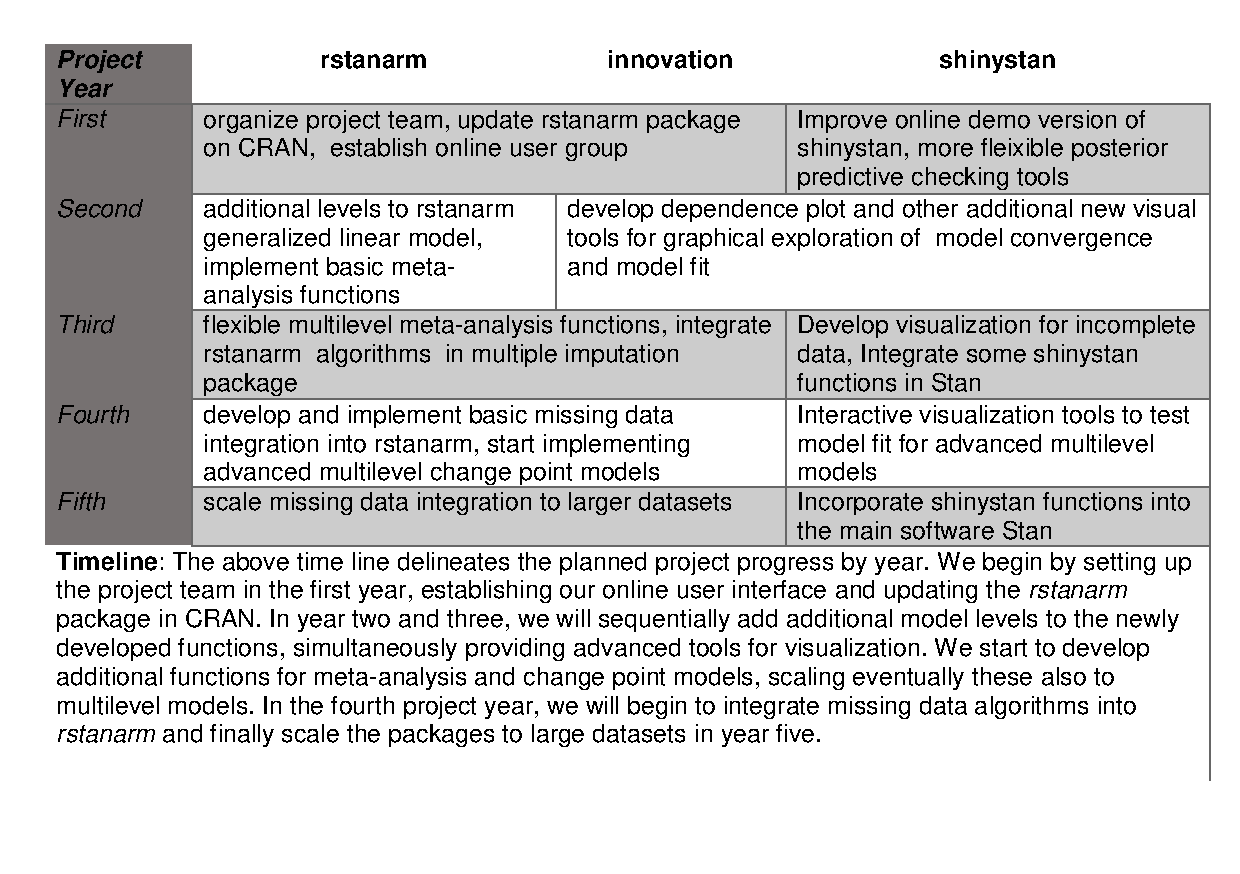
\includegraphics[width=0.7\textwidth]{Figures/Timeline.pdf}
 \vspace{-60pts}
\end{wrapfigure}


Some colleagues are weary to make powerful statistical tools accessible to the initiated ignorant. We counter however that the syntactic simplicity of \textit{rstanarm} will enable more realistic models while rendering the (complex) model structure more transparent. Not only is it ultimately the data scientists' responsibility to specify scientifically reasonable  models correctly reflects the health care delivery data structure design and address meaningful research questions, but also with \textit{rstanarm}, data driven outcomes research will become more transparent and reproducible. Also \textit{shinystan} will contribute to the ease with which advanced hierarchical models and MCMC results can be shared, questioned, discussed and deconstructed.
 


%----------------------------------------------------------------------------------------
%	BIBLIOGRAPHY
%----------------------------------------------------------------------------------------

\newpage

% \nobibliography{K01_bibliography_24Feb15} % to not print a bibiography at the end.
\bibliography{Bibliography/bibliographyBD2K} % the file name cannot contain spaces
\bibliographystyle{Bibliography/nihunsrt} % Use the custom nihunsrt bibliography style included with the template

%----------------------------------------------------------------------------------------

\end{document}
